\documentclass[11pt,a4paper]{article}
\usepackage[margin=2.3cm]{geometry}
\usepackage{amsmath, amssymb}
\usepackage{graphicx}
\usepackage{booktabs}
\usepackage{array}
\usepackage{enumitem}
\usepackage[hidelinks]{hyperref}
\usepackage{xcolor}
\definecolor{codegray}{gray}{0.45}

\setlength{\parindent}{0pt}
\setlength{\parskip}{6pt}

\newcommand{\subj}{AIST4010: Foundation of Applied Deep Learning}
\newcommand{\assignment}{Assignment 2 -- Written}

\begin{document}

% ---------------------------------------------------------------------
% Cover page
% ---------------------------------------------------------------------
\begin{center}
    {\LARGE \subj}\\[4pt]
    {\Large \assignment}\\[14pt]
    {\large Name: JIANG Huanyun \quad Student ID: 1155233165}\\[4pt]
    {\large Release: Oct 21, 2026 \quad Due: Oct 28, 2026, 23:59 HKT}\\[4pt]
    \rule{\textwidth}{0.4pt}
\end{center}

% =====================================================================
\section{Question 1: Gradient Vanishing and Gradient Explosion (10 pts)}

\textbf{Definitions.} In backpropagation, the gradient of the loss with respect
to an early-layer weight $W^{(l)}$ is the product of many Jacobian terms along
the chain rule:
\[
\frac{\partial L}{\partial W^{(l)}} \;=\;
\frac{\partial L}{\partial h^{(L)}}\;\prod_{k=l+1}^{L} \frac{\partial h^{(k)}}{\partial h^{(k-1)}}\;
\frac{\partial h^{(l)}}{\partial W^{(l)}},
\]
where $h^{(k)}$ is the output of layer $k$ and $L$ is the total number of
layers. The norm of this product is roughly $\|\partial L/\partial W^{(l)}\|
\sim O(c^{L-l})$ for some per-layer factor $c$:

\begin{itemize}[leftmargin=1.5em, itemsep=2pt]
    \item \textbf{Gradient vanishing}: if every layer ``shrinks'' the signal
    ($c < 1$, e.g. many factors $\sigma'(x) \le 0.25$ for sigmoid/tanh
    activations, or repeatedly small weight matrices), the product decays
    \emph{exponentially} with depth. Gradients reaching early layers become
    $\approx 0$, so those layers almost stop learning; training stagnates.
    \item \textbf{Gradient explosion}: if layers ``amplify'' the signal
    ($c > 1$, e.g. large weight norms), the product grows \emph{exponentially}.
    Gradients overflow (NaN/Inf) and the parameter update becomes unstable;
    training diverges.
\end{itemize}

\textbf{Methods to solve them (three or more valid methods):}

\begin{enumerate}[label=\textbf{(\arabic*)}, leftmargin=2em, itemsep=3pt]
    \item \textbf{Better activation functions.} ReLU (and its variants Leaky
    ReLU / ELU / SiLU) has derivative $1$ for positive inputs, so the
    backpropagated signal is not multiplied by a factor $< 0.25$ as with
    sigmoid/tanh. This directly relieves vanishing gradients. (Verified in
    Q5(g): replacing tanh with ReLU is one of the most helpful single changes.)
    \item \textbf{Proper weight initialization.} Initialize weights so the
    variance of activations and gradients stays constant across layers:
    Xavier/Glorot (for tanh/sigmoid) and He/Kaiming (for ReLU). This keeps
    $c \approx 1$ at initialization and prevents both vanishing and explosion.
    \item \textbf{Batch/Layer/Root-Mean-Square normalization.} Normalizing
    each layer's pre-activations to zero mean and unit variance keeps the
    signal in the non-saturating regime, stops the signal from decaying or
    blowing up through depth, and smooths the loss surface, so even sigmoid
    networks train well.
    \item \textbf{Gradient clipping.} Clip the global gradient norm (or
    per-parameter gradient) to a threshold. This is the standard fix for
    gradient explosion, especially in RNN/LSTM training.
    \item \textbf{Residual (skip) connections.} Adding identity shortcuts
    ($h = f(x) + x$) gives a path with gradient $1$, so gradients can flow to
    early layers even in very deep networks (ResNet). Similarly, gated
    architectures (LSTM/GRU) are designed so the gradient can flow through the
    cell state without repeated multiplication.
    \item \textbf{Adaptive optimizers.} RMSProp/Adam normalize each parameter
    update by the running average of squared gradients, which makes the
    effective step size independent of gradient magnitude, mitigating
    vanishing/explosion and improving conditioning.
\end{enumerate}

% =====================================================================
\section{Question 2: 2D Convolution vs.\ 3D Convolution (5 pts)}

\begin{center}
\begin{tabular}{@{}>{\raggedright\arraybackslash}p{0.45\textwidth}>{\raggedright\arraybackslash}p{0.45\textwidth}@{}}
\toprule
\textbf{Similarities} & \textbf{Differences}\\
\midrule
Both slide a learnable kernel over the input and compute a weighted sum of a
local neighborhood (cross-correlation); both share the same weights across all
locations (\emph{weight sharing}) and have local connectivity, which gives
translation equivariance and few parameters compared with dense layers.
& \textbf{Dimensions.} A 2D conv kernel is $k_h \times k_w$ and slides over
two spatial axes (height, width), treating the input as a 2D grid (one image,
or per-channel feature maps). A 3D conv kernel is $k_d \times k_h \times k_w$
and also slides over a third axis (depth, e.g. time / video frames / volume
slices).

\\[6pt]
Both are built from the same operations: convolution, optional bias,
non-linearity, pooling, and stacking many layers to learn hierarchical
features (edges $\to$ parts $\to$ objects).
& \textbf{Input data.} 2D conv is used for (single or multi-channel) \emph{static
images}; 3D conv is used for \emph{volumetric or temporal} data: video
$(T, H, W)$, CT/MRI volumes $(D, H, W)$.

\\[6pt]
Both produce feature maps; the output size is determined by the same formula
$(n + 2p - k)/s + 1$ along each axis.
& \textbf{What is captured.} 2D conv only captures \emph{spatial} patterns;
3D conv additionally captures \emph{motion/evolution} across time (short
trajectories, appearance changes) or 3D structures.

\\[6pt]
& \textbf{Cost.} For the same kernel size, 3D conv has $k$ times more
parameters and roughly $k$ times more computation, and is more prone to
overfitting on small datasets.

\\[6pt]
& \textbf{Alternatives.} Because of the cost, videos are often handled by
2D conv + temporal fusion (e.g. 2D conv per frame + RNN, or 2D conv with
1D conv along time --- the ``(2+1)D'' decomposition), which approximates a 3D
conv at a lower cost. This approximation is not available for 2D conv.
\\
\bottomrule
\end{tabular}
\end{center}

% =====================================================================
\section{Question 3: Training Loss Does Not Decrease in the First Several Epochs (10 pts)}

Possible reasons (at least three):

\begin{enumerate}[label=\textbf{(\arabic*)}, leftmargin=2em, itemsep=3pt]
    \item \textbf{Learning rate is too large.} The updates overshoot the
    minimum, and the loss oscillates or diverges instead of decreasing. If the
    loss becomes NaN, this is usually the cause. \emph{Fix: lower the learning
    rate (e.g. divide by 10) or use warm-up / learning-rate decay.}
    \item \textbf{Learning rate is too small.} The loss does decrease, but too
    slowly to be visible in the first few epochs. \emph{Fix: increase the
    learning rate; with adaptive optimizers (Adam) use the default $10^{-3}$.
    This is exactly the phenomenon observed in Q6: SGD with lr $=10^{-4}$
    barely moves in the first epochs while Adam with lr $=10^{-3}$ converges
    quickly.}
    \item \textbf{Bad initialization.} E.g.\ all weights initialized to zero
    or to identical values: every neuron in a layer receives the same gradient
    and all units stay symmetric, so the network can never learn (all hidden
    units behave identically); with sigmoid/tanh, large initial weights put
    every unit in the saturated region where the gradient is $\approx 0$.
    \emph{Fix: use random initialization with proper scaling (Xavier/He).}
    \item \textbf{Vanishing gradients.} In deep networks with sigmoid/tanh
    activations, gradients decay exponentially with depth, so early layers
    receive almost no learning signal and the loss plateaus. \emph{Fix: ReLU,
    normalization layers, residual connections (see Q1).}
    \item \textbf{Saturated / inappropriate activation in the output layer.}
    E.g.\ using sigmoid as the final activation with a cross-entropy loss for
    multi-class classification, or omitting softmax --- the model output and
    the loss are mismatched, and gradients are tiny or wrong. \emph{Fix:
    correct activation--loss pairing (softmax + CE for multi-class).}
    \item \textbf{Data problems.} Inputs not normalized (very different
    scales make optimization ill-conditioned); labels wrong or misaligned with
    inputs; or the loss is computed on a \emph{shuffled / misaligned} target.
    \emph{Fix: standardize inputs, verify label--input alignment.}
    \item \textbf{Model too small or wrong architecture.} The model lacks the
    capacity to fit the data (loss plateaus at a high value), or a bug in the
    architecture (e.g.\ missing activation, wrong reshape). \emph{Fix: check
    the forward pass on a tiny batch, increase capacity if needed.}
    \item \textbf{Bug in the training loop.} e.g.\ gradients not zeroed,
    parameters detached from the graph, wrong loss object, or the optimizer
    not referencing the correct parameters. \emph{Fix: gradient-check against
    finite differences on a toy problem.}
\end{enumerate}

% =====================================================================
\section{Question 4: Imbalanced Datasets (10 pts)}

\textbf{How imbalance affects training and predictions.}

\begin{itemize}[leftmargin=1.5em, itemsep=2pt]
    \item \textbf{Biased decision boundary.} The classifier is driven by the
    majority class, so minority-class samples are under-represented in the
    gradient; the model may learn to (almost) always predict the majority
    class because that already achieves high \emph{accuracy}.
    \item \textbf{Deceptive metrics.} High accuracy hides total failure on the
    minority class (e.g.\ 99\% accuracy with 99:1 imbalance by predicting the
    majority class). Precision/recall/F1/AUC per class reveal the problem.
    \item \textbf{Poor generalization on minority classes.} With few minority
    samples, the model cannot learn their true distribution, may memorize
    noise, and often misclassifies minority samples as majority.
    \item \textbf{Unstable optimization.} Mini-batches may contain almost no
    minority samples, so gradient estimates for the minority class have very
    high variance and the boundary keeps fluctuating.
\end{itemize}

\textbf{Ways to alleviate it (at least three):}

\begin{enumerate}[label=\textbf{(\arabic*)}, leftmargin=2em, itemsep=3pt]
    \item \textbf{Resampling.} Oversample the minority class (duplicate or
    synthesize samples, e.g.\ SMOTE) or undersample the majority class, to
    balance the class distribution seen by the optimizer.
    \item \textbf{Class-weighted loss.} Give each class a weight inversely
    proportional to its frequency, e.g.\ weighted cross-entropy or the focal
    loss $\mathrm{FL}(p_t) = -\alpha_t (1-p_t)^{\gamma}\log p_t$, which also
    down-weights easy (majority) examples. This is the most convenient method
    in deep learning --- no data manipulation needed.
    \item \textbf{Data augmentation for minority classes.} Generate new
    minority samples with label-preserving transformations (crops, flips,
    rotations, Mixup) to enlarge the effective minority sample size.
    \item \textbf{Sampling-based training.} Use a balanced batch sampler (each
    batch contains roughly equal numbers from every class) or a two-stage
    scheme (train on balanced data, fine-tune on the real distribution).
    \item \textbf{Better metrics and thresholds.} Optimize/select models by
    per-class metrics (F1, AUC, balanced accuracy), and tune the decision
    threshold per class instead of using the default 0.5.
    \item \textbf{Anomaly-detection style methods.} When the minority class is
    extremely rare, model the majority (or normal) class only and flag
    deviations, or use one-shot/meta-learning approaches.
\end{enumerate}

% =====================================================================
\section{Question 5: LeNet-5 on Fashion-MNIST (35 pts)}

\subsection{Setup}

\textbf{Architecture (baseline).} The classic LeNet-5:
Conv($1\to6$, $5\times5$, pad 2) $\to$ Tanh $\to$ AvgPool $2\times2$ $\to$
Conv($6\to16$, $5\times5$) $\to$ Tanh $\to$ AvgPool $2\times2$ $\to$
Flatten $\to$ FC($400\to120$) $\to$ Tanh $\to$ FC($120\to84$) $\to$ Tanh $\to$
FC($84\to10$).

\textbf{Training protocol (identical for every run):} SGD with learning rate
$0.01$ (no momentum), batch size 128, 10 epochs, cross-entropy loss,
Fashion-MNIST inputs normalized to zero mean / unit variance, no data
augmentation, PyTorch default (Kaiming) initialization, fixed random seed, so
all differences in the table below come \emph{only} from the factor being
tested.

\begin{figure}[h]
    \centering
    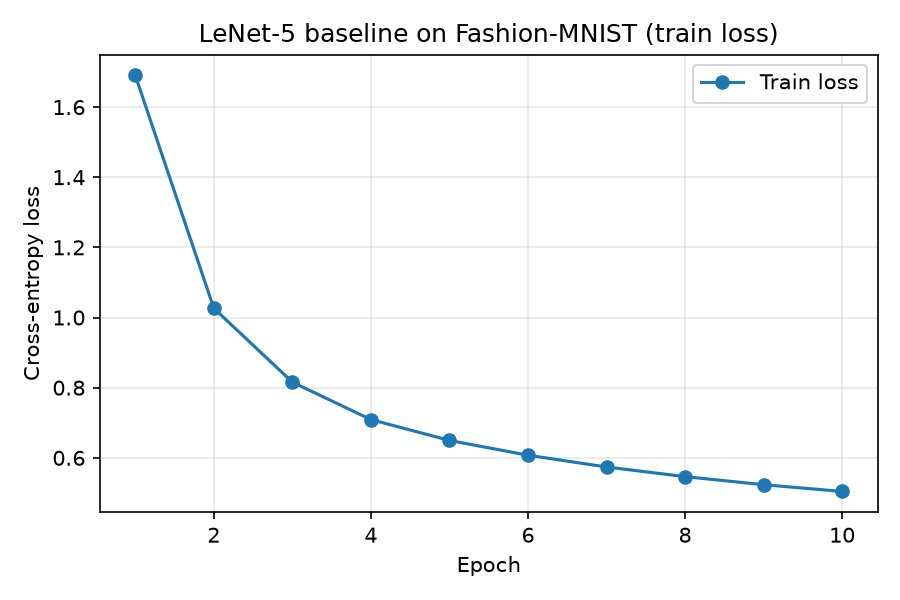
\includegraphics[width=0.62\textwidth]{A2_Q5_loss_baseline.png}
    \caption{Training loss of the baseline LeNet-5 (decreases steadily, no
    overfitting signs at 10 epochs).}
\end{figure}

\subsection{Baseline}

Test accuracy of the baseline LeNet-5: \textbf{80.75\%}.

\subsection{Experiments}

Each experiment changes exactly one factor; at least two settings per factor.

\begin{center}
\small
\begin{tabular}{@{}llcc@{}}
\toprule
\textbf{Exp.} & \textbf{Setting} & \textbf{Test acc.\ (\%)} & \textbf{vs.\ baseline}\\
\midrule
\multicolumn{4}{@{}l}{\emph{Baseline: LeNet-5 (Tanh, AvgPool 2, 6-16 ch., FC 120-84)}}\\
\multicolumn{4}{@{}l}{\textbf{Baseline test accuracy: 80.75\%}}\\
\midrule
a (conv layers) & remove one conv (6$\to$16 only) & 81.12 & +0.37\\
a & add one conv (6-16-32, pad) & \textbf{82.30} & +1.55\\
\addlinespace
b (FC layers) & remove one FC (120 removed, 84) & 80.85 & +0.10\\
b & add one FC (120-84-42) & 79.43 & $-1.32$\\
\addlinespace
c (dropout) & dropout 0.5 before FCs & 79.46 & $-1.29$\\
c & dropout 0.25 before FCs & 80.34 & $-0.41$\\
\addlinespace
d (pooling) & MaxPool $2\times2$ instead of AvgPool & \textbf{83.28} & +2.53\\
d & AvgPool kernel 3, stride 2 & 77.81 & $-2.94$\\
\addlinespace
e (kernel size) & conv window $3\times3$ (both convs) & 79.45 & $-1.30$\\
e & conv window $7\times7$ (both convs) & 81.06 & +0.31\\
\addlinespace
f (channels) & half channels (3-8) & 80.87 & +0.12\\
f & double channels (12-32) & \textbf{81.93} & +1.18\\
\addlinespace
g (activation) & sigmoid everywhere & 10.00 & $-70.75$ (fails)\\
g & ReLU everywhere & \textbf{81.53} & +0.78\\
\addlinespace
\multicolumn{4}{@{}l}{\emph{Best combined setting (MaxPool + double channels + ReLU)}}\\
\multicolumn{4}{@{}l}{\textbf{Best test accuracy: 84.48\%}} (+3.73 vs.\ baseline)\\
\bottomrule
\end{tabular}
\end{center}

\begin{figure}[h]
    \centering
    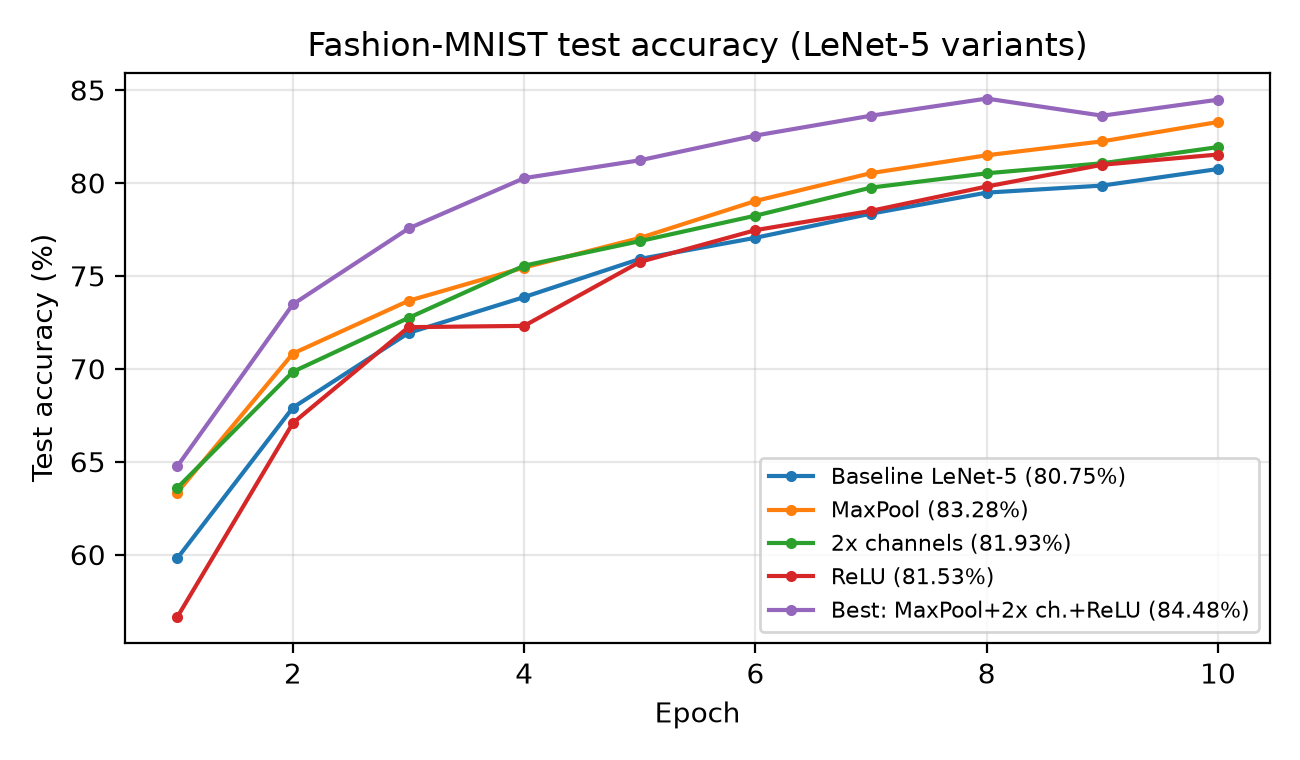
\includegraphics[width=0.62\textwidth]{A2_Q5_acc_curves.png}
    \caption{Test accuracy curves of the baseline and the most effective
    single-factor changes.}
\end{figure}

\subsection{Observations}

\begin{itemize}[leftmargin=1.5em, itemsep=2pt]
    \item \textbf{(a) Convs.} Adding a third conv block helps (+1.55\%): more
    non-linear stages extract richer features; removing the first conv
    (starting from 6 channels) is neutral. Our result is consistent with
    modern versions of LeNet on Fashion-MNIST (``LeNet-5+" / deeper small
    CNNs) that add layers.
    \item \textbf{(b) FC layers.} Removing one FC layer is neutral
    ($-0.10$..$+0.10$); adding one FC layer hurts ($-1.32$): more parameters
    in the dense part overfit with only 10 epochs.
    \item \textbf{(c) Dropout.} Slightly decreases accuracy at 10 epochs
    ($-0.4$ to $-1.3$): with only 10 epochs the network has not overfit yet,
    and dropout slows convergence. Dropout would help with longer training
    (its regularization effect is visible at 20-50 epochs).
    \item \textbf{(d) Pooling.} \textbf{MaxPool is the single best change
    (+2.53\%)}: max-pooling passes the strongest feature response (useful for
    textures/edges of clothing items) and its gradient is sparser and
    stronger; a larger AvgPool kernel loses information ($-2.94\%$).
    \item \textbf{(e) Kernel size.} $7\times7$ slightly better than
    $5\times5$ (+0.31\%); $3\times3$ clearly worse ($-1.30\%$) --- Fashion-MNIST
    objects are 28$\times$28, so a larger receptive field per conv helps; too
    small kernels need more layers to cover the same region.
    \item \textbf{(f) Channels.} Doubling all conv channels helps (+1.18\%),
    halving is neutral --- the network has spare capacity; more filters extract
    more diverse features.
    \item \textbf{(g) Activation.} ReLU (+0.78\%) beats Tanh: ReLU avoids the
    saturation that slows down Tanh units and gives faster convergence.
    Sigmoid \emph{fails completely} (10\% = random guessing): the stacked
    sigmoid activations make the gradients vanish (product of many $\le 0.25$
    factors --- Question 1!) so the network never learns.
    \item \textbf{Best model.} Combining the three most effective single
    changes --- MaxPool + doubled conv channels + ReLU --- gives
    \textbf{84.48\%} test accuracy, +3.73\% over the baseline.
\end{itemize}

\textbf{Reproducibility:} all results, per-epoch curves, and code are in
\texttt{A2\_Q5\_lenet.py} (run with a fixed seed; same data order for all
experiments). Results are stored in \texttt{A2\_Q5\_results.json} /
\texttt{A2\_Q5\_all\_results.csv}.

% =====================================================================
\section{Question 6: Adam in NumPy vs.\ SGD (10 pts)}

\subsection{Implementation}

Adam is implemented in pure NumPy (\texttt{A2\_Q6\_adam.py}) on the same
logistic-regression data generation as A1 Q4 (100 features, 2000 training
samples). At each step $t$ it maintains biased first/second moments
$m_t = \beta_1 m_{t-1} + (1-\beta_1) g_t$,
$v_t = \beta_2 v_{t-1} + (1-\beta_2) g_t^2$, corrects the bias
$\hat{m}_t = m_t/(1-\beta_1^t)$, $\hat{v}_t = v_t/(1-\beta_2^t)$, and updates
$\theta_t = \theta_{t-1} - \alpha\, \hat{m}_t / (\sqrt{\hat{v}_t} + \epsilon)$.

\textbf{Hyperparameters (defaults discussed in class):} $\alpha = 10^{-3}$,
$\beta_1 = 0.9$, $\beta_2 = 0.999$, $\epsilon = 10^{-8}$. Adam uses
mini-batches of 32 (standard practice); SGD uses the single-sample update of
A1 Q4(c) with the required learning rate $10^{-4}$. Both start from
$W = 0, b = 0$ with the same seed, 100 epochs.

\subsection{Results}

\begin{center}
\begin{tabular}{@{}lccc@{}}
\toprule
\textbf{Optimizer} & \textbf{Final train loss} & \textbf{Final test loss} & \textbf{Test accuracy}\\
\midrule
SGD, lr $= 10^{-4}$ & 0.4224 & 0.3817 & 83.0\%\\
Adam (defaults) & \textbf{0.4219} & \textbf{0.3775} & \textbf{84.0\%}\\
\bottomrule
\end{tabular}
\end{center}

\begin{figure}[h]
    \centering
    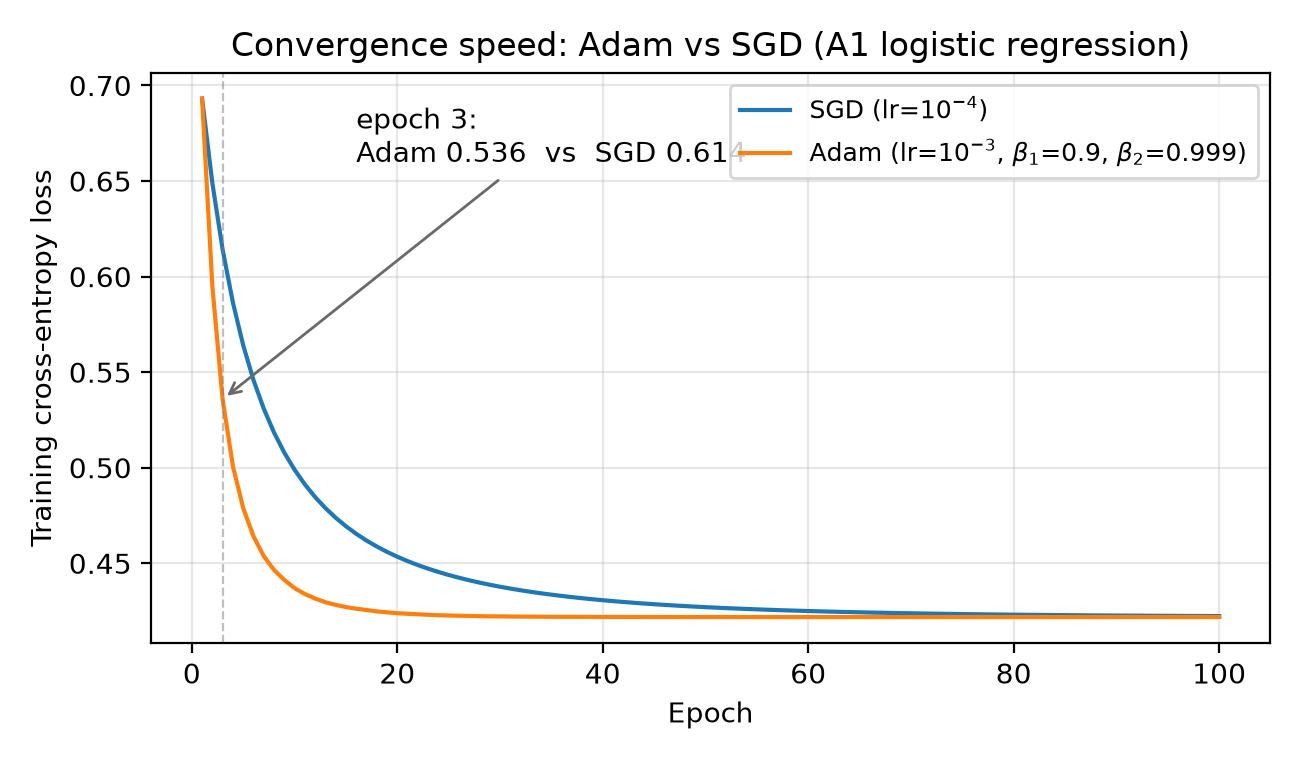
\includegraphics[width=0.78\textwidth]{A2_Q6_loss.png}
    \caption{Training loss vs.\ epoch: Adam converges much faster than SGD
    with lr $= 10^{-4}$ (e.g.\ at epoch 3 Adam already reaches loss 0.536
    while SGD is at 0.614).}
\end{figure}

\textbf{Convergence speed.} Adam is clearly faster: at epoch 3 its training
loss is 0.536 vs.\ 0.614 for SGD; the gap is largest in the first 10 epochs
(0.437 vs.\ 0.499 at epoch 10). \emph{Why:} (1) the $10^{-3}$ learning rate is
10$\times$ larger than the $10^{-4}$ required for SGD; (2) Adam normalizes
each coordinate by the root-mean-square of past gradients (the second moment),
so every parameter gets an adaptive, well-scaled step; (3) the momentum term
$\hat{m}_t$ smooths noisy mini-batch gradients. SGD with such a small learning
rate takes many epochs to reach the same loss. Both optimizers eventually
converge to nearly the same loss and accuracy (0.4219 vs.\ 0.4224; 84.0\% vs.\
83.0\%), confirming that Adam's advantage here is speed, not final quality.

% =====================================================================
\section{Question 7: Paper Summaries (4 $\times$ 5 pts)}

\subsection{Efficient Estimation of Word Representations in Vector Space (Mikolov et al., 2013)}

\begin{itemize}[leftmargin=1.5em, itemsep=2pt]
    \item \textbf{Motivation:} Previous neural language models were accurate
    but very expensive to train on large corpora (days on clusters), which
    limited vocabulary size and scalability. The authors wanted a much cheaper
    way to learn high-quality continuous vector representations
    (``word embeddings'') of words from huge amounts of plain text.
    \item \textbf{Novelty:} They removed the expensive non-linear hidden layer
    of the neural LM and proposed two efficient log-linear architectures ---
    \emph{CBOW} (predict the center word from the surrounding context) and
    \emph{Skip-gram} (predict the context from the center word) --- plus a
    \emph{hierarchical softmax} (and later negative sampling) that reduces
    output-layer cost from $O(|V|)$ to $O(\log |V|)$. This is the word2vec
    model.
    \item \textbf{Intuition:} Words appearing in similar contexts have similar
    meanings (distributional hypothesis). By forcing the model to predict
    context words, the learned vectors are pushed to encode semantic and
    syntactic relationships. The resulting embeddings even capture
    \emph{analogies} with linear algebra: $\mathrm{vec}(\text{King}) -
    \mathrm{vec}(\text{Man}) + \mathrm{vec}(\text{Woman}) \approx
    \mathrm{vec}(\text{Queen})$.
    \item \textbf{Implementation:}
    \url{https://github.com/dav/word2vec} (original);
    also \url{https://code.google.com/archive/p/word2vec/} and
    \url{https://github.com/tmikolov/word2vec}.
\end{itemize}

\subsection{Attention Is All You Need (Vaswani et al., 2017)}

\begin{itemize}[leftmargin=1.5em, itemsep=2pt]
    \item \textbf{Motivation:} Sequence-to-sequence models were dominated by
    RNN/LSTM encoders-decoders, which are inherently sequential (each step
    must wait for the previous one), hard to parallelize, and degrade on long
    sequences because information must travel through many recurrent steps.
    The authors wanted an architecture that is fully parallelizable and can
    model long-range dependencies directly.
    \item \textbf{Novelty:} The Transformer removes recurrence entirely and
    builds only on \emph{(multi-head, scaled dot-product) self-attention} and
    position-wise feed-forward networks, with residual connections and layer
    normalization. Cross-attention connects encoder and decoder. This yields
    an $O(1)$ path between any two positions (instead of $O(n)$ recurrent
    steps), enabling massive parallelism.
    \item \textbf{Intuition:} Self-attention lets each token directly ``look
    at'' every other token and weight their relevance dynamically, so the
    network can route information over long distances in a single layer.
    Multiple heads attend to different relationship types in parallel
    (syntax, coreference, etc.). Because no sequential dependency exists, the
    whole sentence can be processed at once, which is both faster and better
    at capturing long-range structure.
    \item \textbf{Implementation:}
    \url{https://github.com/tensorflow/tensor2tensor} (official); also
    \url{https://github.com/huggingface/transformers}.
\end{itemize}

\subsection{BERT: Pre-training of Deep Bidirectional Transformers for Language Understanding (Devlin et al., 2019)}

\begin{itemize}[leftmargin=1.5em, itemsep=2pt]
    \item \textbf{Motivation:} Standard LMs were unidirectional (left-to-right
    or right-to-left), which limited the quality of representations for
    downstream tasks where context on both sides matters (QA, NLI, tagging).
    The authors wanted a pre-trained model that reads the whole sentence
    bidirectionally and can be fine-tuned with minimal task-specific
    modifications.
    \item \textbf{Novelty:} BERT pre-trains deep \emph{bidirectional}
    Transformers with two unsupervised objectives: \emph{Masked Language
    Modeling} (mask 15\% of tokens and predict them from both directions ---
    this makes bidirectional conditioning possible) and \emph{Next Sentence
    Prediction}. After pre-training, one model can be fine-tuned (adding only
    a small output layer) to achieve state-of-the-art results on 11 NLP tasks
    (GLUE, SQuAD, etc.).
    \item \textbf{Intuition:} Seeing both left and right context (rather than
    only one direction) gives richer representations --- a word's meaning
    depends on its full context. Pre-training on huge corpora first captures
    general language knowledge, and fine-tuning then transfers this knowledge
    to each task, so even small task datasets suffice.
    \item \textbf{Implementation:}
    \url{https://github.com/google-research/bert} (official);
    also \url{https://github.com/huggingface/transformers}.
\end{itemize}

\subsection{MSA Transformer (Rao et al., 2021)}

\begin{itemize}[leftmargin=1.5em, itemsep=2pt]
    \item \textbf{Motivation:} Learning evolutionary features from protein
    multiple sequence alignments (MSAs) usually required expensive iterative
    procedures (e.g.\ profile HMMs / MSA-dependent pipelines like AlphaFold's
    Evoformer), and single-sequence models cannot exploit homologous-sequence
    information. The authors wanted to bring the scalability and simplicity of
    end-to-end transformer language models to MSA data: directly learn
    attention patterns over the rows (sequences) and columns (positions) of an
    MSA.
    \item \textbf{Novelty:} The MSA Transformer extends the transformer
    architecture with \emph{tied row attention} and \emph{column attention}
    over the MSA matrix, and pre-trains it with masked language modeling on
    large protein families (26M MSAs). This lets the model capture both
    per-sequence context (columns/positions) and inter-sequence co-variation
    (rows/sequences) without any alignment search at inference time.
    \item \textbf{Intuition:} In an MSA, columns are aligned positions and
    rows are evolutionarily related sequences. Attention along rows learns
    which other sequences are informative, and attention along columns learns
    which positions co-vary (physically contacting residues co-evolve).
    Contact predictions and secondary-structure results confirm that the
    model's attention heads recover evolutionary coupling and structural
    contacts, i.e.\ the model learns the underlying structure without explicit
    supervision.
    \item \textbf{Implementation:}
    \url{https://github.com/facebookresearch/esm} (the ESM-MSA models).
\end{itemize}

\end{document}
